\documentclass[12pt]{phys-thesis}

\usepackage[utf8]{inputenc}
\usepackage[letterpaper,bindingoffset=0.2in,left=1in,right=1in,top=1in,bottom=1in,footskip=.25in]{geometry}

\usepackage[style=phys]{biblatex} % biblatex with aps physics style citations
\addbibresource{main.bib}

\usepackage{amsmath}
\usepackage{amssymb}
\usepackage{graphicx}
\usepackage{dsfont} % some special charaters
\usepackage{rotating}

% for inserting stuff into toc manually
\usepackage{tocloft}

% tables and such
\usepackage{tabularx}
\usepackage{booktabs}

% header and footer stuff
\usepackage{fancyhdr}
\renewcommand{\headrulewidth}{0pt}

%\usepackage{hyperref}
\fancyhf{}
\fancyhead[R]{\thepage}
\pagestyle{fancy}
% Redefine the plain page style, which chapters use
% so that there is a number on chapter pages
\fancypagestyle{plain}{%
  \fancyhf{}%
  \fancyhead[R]{\thepage}
}

\usepackage{hyperref}
\hypersetup{
  colorlinks=true,
  linkcolor=blue,
  citecolor=blue,
  urlcolor=blue,
}

% double spacing
\usepackage{setspace}
\doublespacing

% define how equations and figures are called in the whole document
% i.e. Eqn or Eqn. or Equation etc...
\newcommand{\eqn}[1]{Equation \ref{#1}}
\newcommand{\fig}[1]{Figure \ref{#1}}
\newcommand{\sect}[1]{Section \ref{#1}}

\newcommand{\W}{\ensuremath{\mathcal{W}}}
\newcommand{\bbar}{\ensuremath{|\bar{1}\rangle}}

% dont make italicized
\DeclareMathOperator\erf{erf}

\begin{document}
\pagenumbering{roman} % roman numerals before main content

\include{abstract}

\include{acknowledgements}


\title{Neutral Atom Ensemble Qubits and Rydberg Blockade}
\author{Matthew F Ebert}
\newcommand{\oraldate}{1/31/2017}% change to the defense date
\newcommand{\profA}{Iam A. Professor, Professor, Geography}
\newcommand{\profB}{Iam A. Professor, Professor, Geography}
\newcommand{\profC}{Iam A. Professor, Professor, Geography}
\newcommand{\profD}{Iam A. Professor, Professor, Geography}
\newcommand{\profE}{Iam A. Professor, Professor, Geography}
\date{\today{}}

\maketitle

\begin{dedication}
  To someone
\end{dedication}

\begin{abstract}
  this is an abstract
\end{abstract}

\tableofcontents

%\listoffigures



\pagenumbering{arabic} % arabic numerals for main content

\graphicspath{{introduction/figures/}}
\chapter{Introduction}\label{ch_intro}

Ensemble qubits are systems, composed of constituent sub-systems, where quantum information can be encoded in one or more effective two-state qubits\cite{LukinFleischhauerCoteEtAl2001,Brion2007}, see \fig{fig_ensemblegen}.
In the particular neutral atom implementation described in this work, an ensemble qubit is a collection of atoms that are manipulated in a way where the individual atoms are identicle, not resolvable, and addressed by external fields simultaneously.
In atom implementations, information is typically encoded in the hyperfine manifold of the ground state of the sub-systems, as these states are well isolated from environmental decoherence effects, which degrade the performance of the system.

\begin{figure}
  \centering
  \label{fig_ensemblegen}
  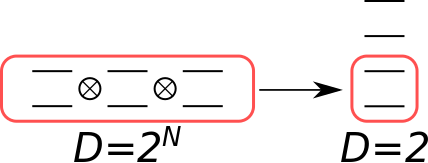
\includegraphics[width=0.5\textwidth]{ensemble_general}
  \caption{
    A diagram of an ensemble qubit composed of $N=3$ constituent two-state systems.
    In the ensemble, the maximum energy of the system is restricted to a single excitation.
    Information is stored in the lowest energy levels of the ensemble qubit only.
  }
\end{figure}

While ensemble qubits add some complex considerations like collisional decoherence channels, there are significant advantages that make ensembles a convienent qubit implementation.
Deterministically preparing an array of single atoms quickly, simply, and efficiently is an outstanding problem in the field\cite{583606310,BakrPengTaiEtAl2010,Endres2016,Barredo1021,SerwaneZuernLompeEtAl2011}, whereas deterministically preparing an ensemble of atoms with $N>1$ in every site in an array is a standard practice, requiring no additional complexity.
With information encoded in an ensemble, trap loss events are not a critical error, as with single atom qubits, and information can be recovered with an appropriate error correction scheme\cite{Brion2007}.
Finally, the ensemble experiences an increased coupling to a particular propagation mode of the light field enabling quantum repeater protocols with no external cavity enhancement\cite{Pedersen2009}.

There are many quantum information and communication schemes developed for ensemble systems, a few schemes that are relevent to our implementation will be discussed here.
This work will focus on cataloging the progress made in developing a Rydberg interaction mediated ensemble qubit architecture for use in these applications.

\section{Ensemble Qubit Protocols}
All the qubit protocols discussed utilize the "Rydberg blockade" phenomenon to provide a controllable interaction between qubits 12-orders of mangitude larger than interactions between ground state atoms\cite{SaffmanWalkerMolmer2010}, \fig{fig_rydinteract}.
Rydberg blockade is a molecular dipole-dipole interaction between atoms in highly excited principle quantum number states $n$.
\begin{figure}
  \centering
  \label{fig_rydinteract}
  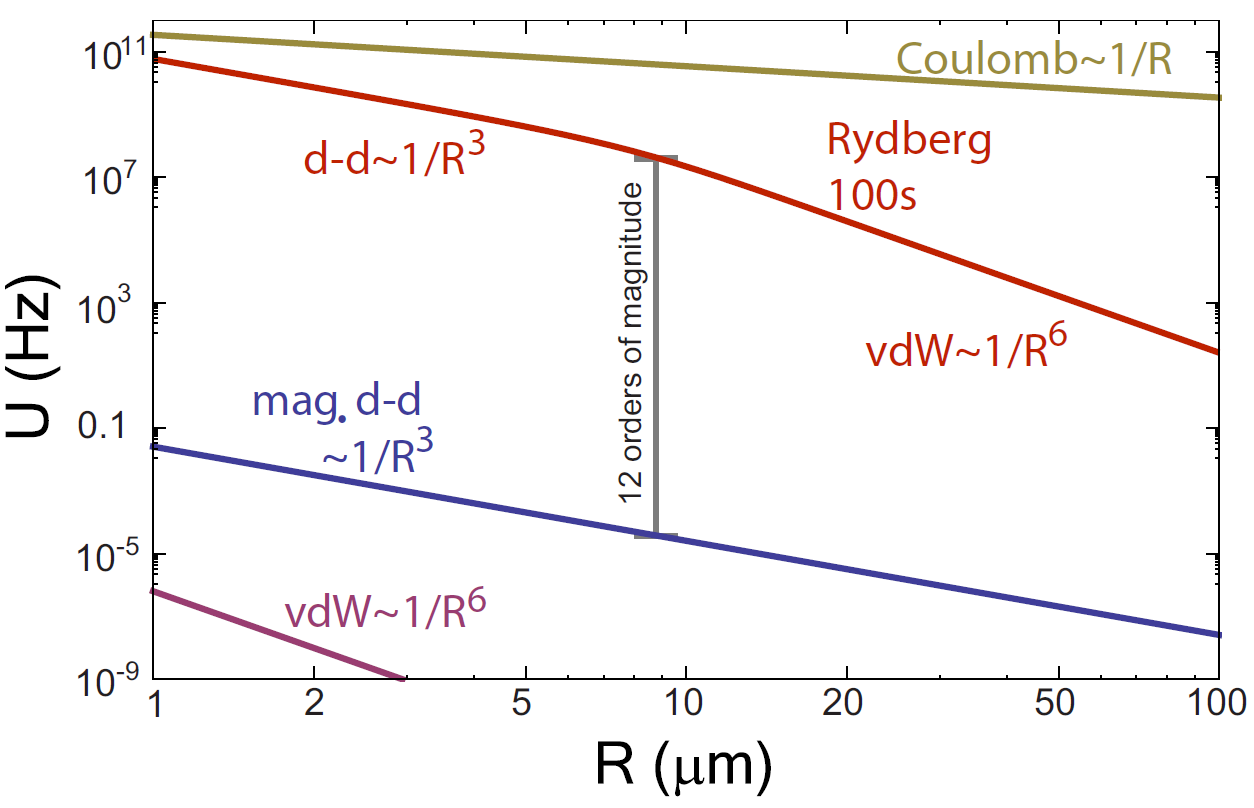
\includegraphics[width=0.6\textwidth]{RydbergInteractions}
  \caption{
    Figure is taken from reference \cite{SaffmanWalkerMolmer2010}, and shows the scale of the relative molecular interaction strengths at some interatomic distance ($R$) between ground state atom pairs (van der Waals and magnetic dipole-dipole interations), Rydberg atom pairs (electric dipole-dipole interations), and ion pairs (Coulomb interactions).
    The Rydberg interaction goes as $R^{-3}$ at short range in the F\"{o}ster regime and $R^{-6}$ in the van der Waals regime at larger separation.
  }
\end{figure}
An interaction energy shift, $\Delta_{dd}$, on the order of the Rabi frequency of the Rydberg excitation, $\Omega$, suppresses the excitation of double Rydberg excited states, $|rr\rangle$, due to the off-resonant excitation energy.
In the strong interaction limit, $\Delta_{dd} \gg \Omega$, the excitation of $|rr\rangle$ is negligible and effectively reduces the Hilbert space of the problem to a two-state system with a collective basis, denoted in this work by $\{|\bar{0}\rangle,|\bar{r}\rangle\}$.
The $|\bar{0}\rangle\equiv|0^{(1)}...0^{(n)}\rangle$ state is the product state with all atoms in the ensemble in the initial non-interacting ground hyperfine state $|0\rangle$.
The $|\bar{r}\rangle$ state is the entangled collective symmetric singly excited state of the ensemble, known as the \W{}-state\cite{DuerVidalCirac2000}, and is defined as:
\begin{equation}
  \label{eq_wstate}
  |\W{}\rangle \equiv |\bar{r}\rangle = \frac{1}{\sqrt{N}}\sum_{k=1}^{N}|0^{(1)}...r^{(k)}...0^{(N)}\rangle,
\end{equation}
where $|r^{(k)}\rangle$ is the Rydberg state of the $k^{\mathrm{th}}$ atom in the ensemble.
The Rydberg state has a short lifetime, $T_1\sim300$ $\mu$s for $n=100$\cite{SaffmanWalkerMolmer2010}, relative to the lifetime of the ground hyperfind manifold and is sensitive to external fields, and therefore it is necessary to map the Rydberg population to the $|\bar{1}\rangle$ state, which is a state in the other ground hyperfine manifold from $|0\rangle$.

Protocols using Ryberg interaction mediated ensemble qubits differ from single atom qubit protocols in the implementation of local rotations.
In typical single atom qubit local rotations, a Raman laser or microwave is used to drive transistions between qubit states\cite{IsenhowerUrbanZhangEtAl2010}.
However in the case of ensemble qubits, local rotations must be done through the Rydberg state to preserve control of excitation number, which encodes the state of the qubit.
This means every ensemble qubit protocol will begin and end with a $\pi$ rotation, $R_1(\pi)$, $|1\rangle \leftrightarrow |r\rangle$ so that the state of the qubit is stored in the "storage basis" $\{|\bar{0}\rangle,|\bar{1}\rangle\}$, but all gates occur in the "computational basis" $\{|\bar{0}\rangle,|\bar{r}\rangle\}$.
A single qubit rotation with angle $\theta$ and phase $\phi$ between $|\bar{0}\rangle$ and $|\bar{1}\rangle$ is implemented by:
$$|\psi'\rangle=R_1(\pi)R_0(\theta,\psi)R_1(\pi)|\psi\rangle.$$
A two-qubit $C_Z$ gate between control and ensemble qubits $C,T$ is implemented by:
$$|\psi'\rangle=R^{(C)}_1(\pi)R^{(T)}_1(2\pi)R^{(C)}_1(\pi)|\psi\rangle.$$

\begin{figure}
  \centering
  \label{fig_ensembleproto}
  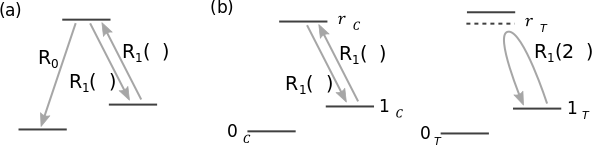
\includegraphics[width=1.0\textwidth]{EnsembleProcedures}
  \caption{
    Gate protocols ensemble qubit schemes for (a) a Haddamard gate and (b) a $C_Z$ two-qubit gate.
  }
\end{figure}

Encoding multiple qubits into the different magnetic hyperfine sub-levels of an ensemble has been proposed as an extension of the basic protocol discribed previously\cite{LukinFleischhauerCoteEtAl2001,Brion2007}.
Here the storage basis is the excitation number in each of the hyperfine sub-levels, while the computational basis requires at least two separate Rydberg states to be used to prevent mixing since all qubits are spatially indistinguishable, and therefore must be spectrally multiplexed.

\section{Quantum Communication with Ensembles}
The distribution of quantum information between non-local nodes has interesting applications, such as distributed quantum computing\cite{Duan2004,Jiang2007}, sensing, metrology\cite{Komar2014,Komar2016}, and cryptography\cite{PhysRevLett.67.661}.
The Ekert protocol requires direct transmission of a photonic (or equivalent) qubit to generate remote entanglement between nodes.
Since loss mechanisms in a distribution channel are exponential there is a practical limit imposed on the distribution radius of the quantum information, due to exponentially growing resource requirements.
For light in a telecom fiber the length scale is $\sim 100$ km.

Quantum repeaters, such as the DLCZ protocol\cite{DLCZ2001}, can extend the range of these quantum networks on lossy channels, using heralded entanglement schemes and reducing the loss to polynomic.
The DLCZ scheme is implemented by probabilistically generating entanglement, through a short collective excitation, between the internal state of both memory qubits at each node with a photonic qubit.
The photons are directed to be incident on a 50/50 beamsplitter, such that detection of a photon on either detector does not determine the source of the photon.
A measurement of a photon on either detector heralds the creation of an entangled state of the two remote node memory qubits with state: $|\psi\rangle=\frac{1}{\sqrt{2}}\left(|\bar{0}_L\rangle|\bar{1}_R\rangle+e^{i\phi}|\bar{1}_L\rangle|\bar{0}_R\rangle\right)$.

Since the DLCZ scheme relies on the production of the collective symmetric singly excited state ($\bbar$) of the ensemble with negligible double excitation probability, incorporation of Rydberg blockade is a clear improvement over the original probabilistic scheme.
With some changes to the protocol, a two-photon coincidence event heralds the creation of remotely entangled nodes at significantly higher rates\cite{Zhao2010,Han2010}.
Incorporation of quantum error correction protocols at the intermediate nodes further improves the rate of entanlgement generation\cite{Fowler2010}.
Since Rydberg blockade can be used to generate entanglement, directional single photon emission, and perform error correction routines it stands as a strong candidate for a quantum communication architecture, even at current entanglement generation fidelities.
Recent demonstrations of photon-ensemble entanglement\cite{LiDudinKuzmich2013}, Rydberg blockade between ensemble qubits, and quantum memory lifetimes of a few ms\cite{EbertKwonWalkerEtAl2015} lay the groundwork for the demonstration of a simple Rydberg-mediated DLCZ based quantum repeater in the near future\cite{Solmeyer2016}.

\section{The \W{}-state}
The \W{}-state, or \bbar{}, is an entangled state of $N$ two-state systems defined by \eqn{eq_wstate}.
Creation of the \bbar{} state can be accomplished stochastically, via a short excitation pulse\cite{Haas180}, or deterministically, using a process that limits the Hilbert space of the ensemble.
By performing an excitation to the Rydberg state under strong blockade conditions, the effective Hilbert space is limited to $|\bar{0}\rangle \equiv |0^{(1)}...0^{(N)}\rangle$ and \bbar{} (ignoring effects of inhomogeneous broadening), which allows for deterministic preparation of \bbar{}.

Some of the properties of the \bbar{} state are non-intutive to those familiar with a typical non-interacting ensemble, and it is helpful to demonstrate some fundamental properties.
We will consider the system to consist of $N$ spin $1/2$ particles, $|0(1)\rangle\rightarrow|-(+)\rangle$, and will investigate the problem in two bases: the internal state basis ($ |\pm^{(1)}\rangle \otimes |\pm^{(2)}\rangle \otimes ... |\pm^{(N)}\rangle$) and the Dicke basis ($|JM\rangle$).
For more information, the interested reader should refer to \cite{Arecchi1972}.

\subsection{Internal State Basis}\label{sec_idealmodel}
The interaction of a generic ensemble excitation with a light field can be written in the basis of individual atom excitations ($ |\pm^{(1)}\rangle \otimes |\pm^{(2)}\rangle \otimes ... |\pm^{(N)}\rangle$).
The interaction Hamiltonian, $\mathbf{H}_{int}$, describing the evolution of the system is a block tridiagonal matrix where the basis states associated with main block diagonals, $\mathbf{\Delta}_{n}$, are degenerate under the excitation Fock state operator, $\hat{\cal{N}} \equiv \sum_{k=1}^N \hat{S}_z^{(k)} + N/2$, where $\hat{S}_{\mu}^{(k)}=\frac{1}{2}\hat{\sigma}_{\mu}^{(k)}$ is the spin projection operator along the axis defined by $\mu$.
The basis states of the system are denoted as $|n_k\rangle$, where $n$ denotes the eigenvalue of $\hat{\cal{N}}$ and the index $k$ breaks the degeneracy of the operator, e.g. $|1_1\rangle=|+-\cdots -\rangle$ and $|2_1\rangle = |++-\cdots -\rangle$.
The matricies on the other diagonals couple the system between excitation number state, i.e. a double excitation occurs by coupling a singly excited state, $|1_k\rangle$ to a doubly excited state $|2_j\rangle$, instead of second order process directly from the ground state.
In this basis $\mathbf{H}_{int}$ is given by:
\begin{equation}
  \label{eqn_blocktridiagonal}
  \begin{split}
    &\mathbf{H}_{int} = \mathbf{A} + \mathbf{\Delta} = \\
    &\begin{bmatrix}
      \mathbf{\Delta}_{0} & \mathbf{A}_{(0,1)} & 0 & & \cdots & & 0 \\
      \mathbf{A}^{T}_{(0,1)} & \mathbf{\Delta}_{1} & \mathbf{A}_{(1,2)} & & & & \\
      0 & \ddots & \ddots & \ddots & & & \vdots \\
        & & \mathbf{A}^{T}_{(n-1,n)} & \mathbf{\Delta}_{n} & \mathbf{A}_{(n,n+1)} & & \\
      \vdots & & & \ddots & \ddots & \ddots & 0 \\
        & &        & & \mathbf{A}^{T}_{(N-2,N-1)} & \mathbf{\Delta}_{N-1} & \mathbf{A}_{(N-1,N)}   \\
      0 & & \cdots & & 0 & \mathbf{A}^{T}_{(N-1,N)} & \mathbf{\Delta}_{N}
    \end{bmatrix}
  \end{split}
\end{equation}
The matrix $\mathbf{H}_{int}$ dimension is $2^N$, the dimension of $N$ 2-level systems.
The dimension of the block diagonal sub-matricies is given by the binomial coefficient, $\textrm{dim}\left( \mathbf{\Delta}_n \right) = \tbinom N{n} \equiv N_{n}$.
The block diagonal sub-matricies, $\mathbf{\Delta}_{n}$, contain information concerning the sub-system's specific energy levels.
\begin{equation}
  \label{eqn_bdsubmatricieselem}
  \mathbf{\Delta}_{n} = \sum_{k=1}^{N_{n}}\delta_{k}^{(n)} |n_k\rangle\langle n_k| +
  \sum_{k=1}^{N_{n}}\sum_{j=1,\neq k}^{N_{n}}\omega_{(j,k)}^{(n)}/2|n_k\rangle\langle n_j|,
\end{equation}
\begin{equation}
  \label{eqn_bdsubmatricies}
  \mathbf{\Delta}_{n} = \begin{bmatrix}
    \delta^{(n)}_1 & \omega^{(n)}_{(1,2)}/2 & \cdots & \omega^{(n)}_{(1,{N_{n}})}/2 \\
    \omega^{(n)}_{(2,1)}/2  & \delta^{(n)}_2 & \cdots & \omega^{(n)}_{(2,{N_{n}})}/2 \\
    \vdots                  & \vdots                    & \ddots & \vdots         \\
    \omega^{(n)}_{({N_{n}},1)}/2  & \omega^{(n)}_{({N_{n}},2)}/2    & \cdots & \delta^{(n)}_{N_n}

  \end{bmatrix},
\end{equation}
where $\delta^{(n)}_k$ refers to the energy of the $k^{\mathrm{th}}$ basis state in the subspace with eigenvalue $n$.
Likewise, $\omega^{(n)}_{(i,j)}$ is the Rabi frequency for excitation hopping from basis state $|n_i\rangle$ to $|n_j\rangle$, the analysis of which is outside the scope of this thesis.

The coupling sub-matricies, $\mathbf{A}_{(n,n +1)}$, contain the specfic coupling strength between each subsystem's spin up and down states, $|-^{(k)}\rangle \leftrightarrow^{\alpha_k} |+^{(k)}\rangle$.
The matrix elements are given by:
\begin{equation}
  \label{eqn_couplingsubmatricies}
  \left[\mathbf{A}_{(n,n +1)}\right]_{(i,j)} = |(n +1)_i\rangle\langle (n +1)_i|\hat{A}|n_j\rangle\langle n_j|,
\end{equation}
where the operator $\hat{A}$ is given by:
\begin{equation}
  \label{eqn_aop}
  \hat{A} = \sum_{k=1}^{N} \alpha_k \left( \mathds{1}^{\otimes (N-1)} \otimes \hat{S}_x^{(k)}\right).
\end{equation}
In other words, two states only have non-zero coupling martix elements if they differ only in the excitation state of a single sub-system.

It is convenient to investigate inhomogeneous effects and system-specific couplings using this formalism, but some important physics is obfuscated.
For example, perfect Rydberg blockade can be implemented by removing all states with $n > 1$, dramatically reducing the size of the dimension of the problem from $2^n$ to $n+1$.
Near perfect blockade can also be implemented by removing $n > 2$ and adding in the interaction energies to $\mathbf{\Delta}_2$.
For more detail the reader is refered to \sect{sect_ensemblemodeling}.

For a first attempt at modeling the system, consider the homogeneous case where $\left[\mathbf{\Delta}_{n}\right]_{(i,j)}=0$ and $\alpha = \alpha_i$.
This is a typical model for a non-interacting ensemble, and therefore we should intuitively expect to observe full inversion of the atomic populaton from the ground to the excited state for all $N$ atoms.
The time evolution of this system is plotted in \fig{fig_compositehomo} for different observables $|\langle n|\psi(t)\rangle|^2$(a), $\langle\hat{N}(t)\rangle$(b), and should be familiar.
\begin{figure}
  \label{fig_compositehomo}
  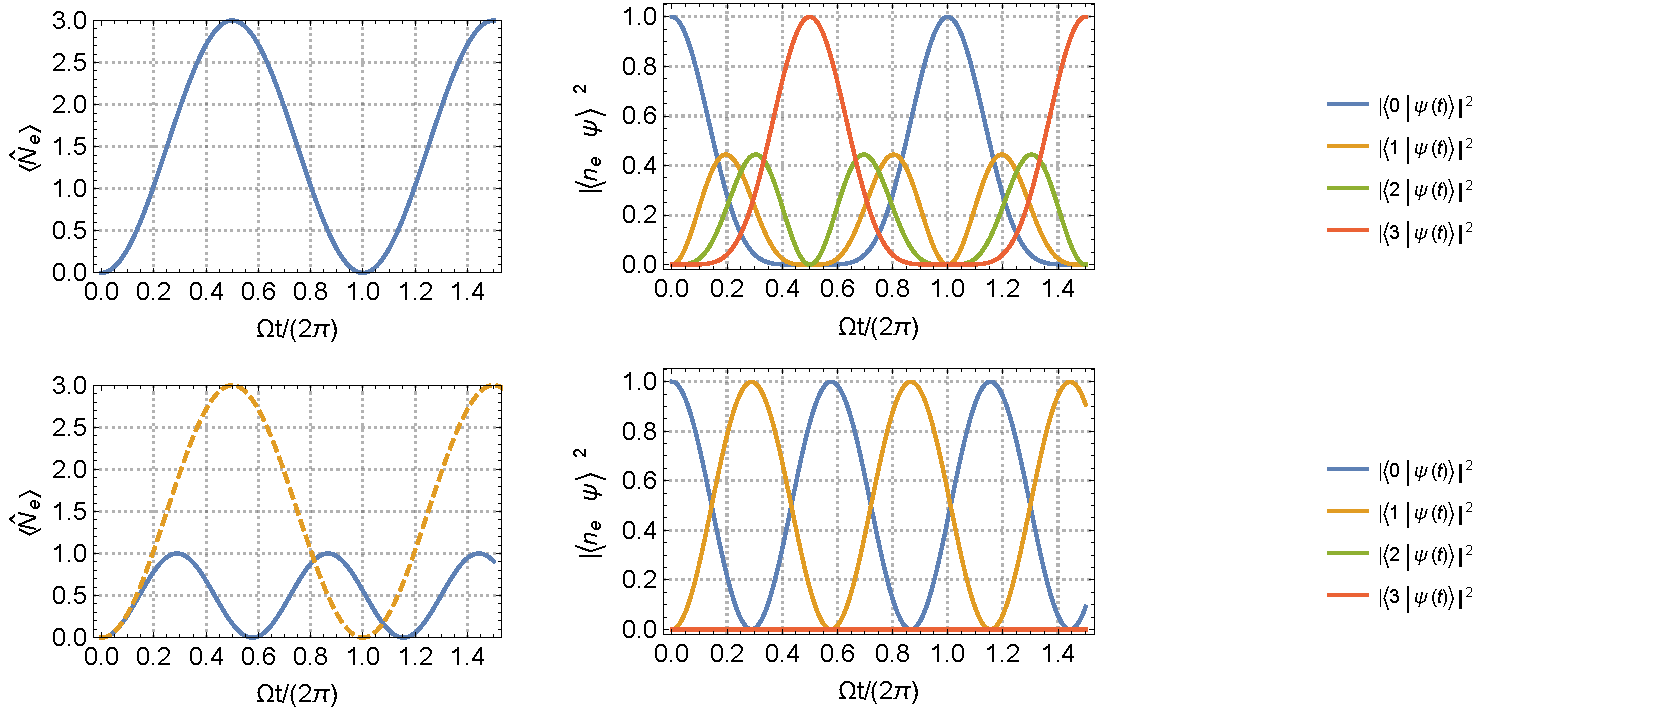
\includegraphics[width=1.0\textwidth]{unblockaded_RFE}
  \caption{
    Example homogeneous (a,b) and blockaded (c,d) Rabi oscillations with $N=3$ atoms with inital state $|\bar{0}\rangle$.
    (a) The average excitation number and (b) the excitation Fock state probabilities as a function of coupling time for an uncoupled sample.
    (c) The average excitation number and (d) the excitation Fock state probabilities as a function of coupling time for a blockaded sample.
  }
\end{figure}

By including a blockade shift, $\delta^{(n>1)}_k = \delta_{dd} >> \alpha$, the Hilbert space of the problem is reduced to $n=\{0,1\}$, and $\mathbf{H}_{int}$ becomes:
\begin{equation}
  \label{eqn_hintsimp}
  \mathbf{H}_{int} = \begin{bmatrix}
    0 & \alpha_1 & \alpha_2 & \cdots & \alpha_N \\
    \alpha_1 & \delta_1^{(1)} & 0 & \cdots & 0 \\
    \alpha_2 & 0 & \delta_2^{(1)} &  & 0 \\
    \vdots & \vdots & & \ddots  & \vdots \\
    \alpha_N & 0 & 0 & \cdots & \delta_N^{(1)} 
  \end{bmatrix}
\end{equation}
The detunings $\delta_k^{(1)}$ are nominally 0, so it makes sense to treat the $\delta^{(1)}$ entries as a perturbation.
Under the condition of perfect blockade, the energy eigenstates of $\mathbf{A}$ are the 2 dressed states with total angular momentum $J = N/2$, $\frac{1}{\sqrt{2}}\left(|\bar{0}\rangle \pm |\bar{1}\rangle\right)$, and the $N-1$ orthogonal states with $J = (N/2 -1)$: $|(\bar{1})_{\perp}\rangle\}$, where $|\bar{1}\rangle \equiv \sum_{k=1}^N \frac{\alpha_k}{\alpha_N}|1^{(k)}\rangle$ and $\alpha_N^2 \equiv \sum_{k=1}^N \alpha_k^2$.
If the initial state is $|\bar{0}\rangle$, then the system will remain in the symmetric subspace defined by $\{|\bar{0}\rangle,\bbar{}\}$.
The eigenvalues determine the speed that population amplitudes will oscillate, for $\frac{1}{\sqrt{2}}\left(|\bar{0}\rangle \pm |\bar{1}\rangle\right)$ this speed is $\pm \alpha_N$ implying a collective enhancement of $\sqrt{N}\alpha$ with homogeneous coupling strengths, see \fig{fig_compositehomo}(c,d).
The collective enhancement of the Rabi frequency is the hallmark of a strongly blockaded ensemble\cite{GaeetanMiroshnychenkoWilkEtAl2009,DudinLiBarianiEtAl2012,Ebert2014,Zeiher2015}.

\subsection{Dicke Basis}\label{sec_jm}
If the homogeneous problem is reformulated in the total angular momentum basis $|J,M\rangle$, it is compartively easier to see the collective Rabi frequency enhancement.
In this basis the quantum numbers that describe the system are the total angular momentum $J$, with associated operator $\hat{J}^2=\hat{J}_x^2+\hat{J}_y^2+\hat{J}_z^2$, where $\hat{J}_{\mu}=\sum_{k=1}^N \hat{S}_{\mu}^{(k)}$, and $M$ is the eigenvalue of the $\hat{J}_z$ operator.
The interaction Hamiltonian is still given by $\mathbf{H}_{int} = \mathbf{A} + \mathbf{\Delta}$, and since $\mathbf{A}$ cannot couple states of unequal angular momentum the evolution of the system is constrained to $J=J(t=0)$, to the extent that $\mathbf{\Delta}$ is negligible.
The typical initialization condition is $|\psi(t=0)\rangle = |\bar{0}\rangle \equiv |N/2,-N/2\rangle$ which can only evolve into state with the maximum total angular momentum.
The Dicke states $|J=N/2,M\rangle=|M\rangle$ are equivalent to the set of $N+1$ symmetric states $\{|\bar{0}\rangle, \bbar{}, |\bar{2}\rangle, \cdots, |\bar{N}\rangle\}$.
When a binary interaction energy sufficient to neglect double excitations is included as before, we are left only with the $|-N/2\rangle = |\bar{0}\rangle$ and $|-N/2+1\rangle = \bbar{}$ states which form an effective 2-state system for the ensemble.

Explicitly, the Hamiltonian in the Dicke basis is given by:
\begin{equation}
  H = \sum_{k=-J}^{J}\delta_k|k\rangle\langle k| 
  + \frac{\alpha}{2}\sum_{m=-J}^{J} \sqrt{\left(J-m+1\right)\left(m+J\right)}\bigg(|m-1\rangle\langle m| + |m\rangle\langle m-1|\bigg).
\end{equation}
This exactly reproduces the results of the substantially larger dimensional system, for the homogeneous case with initial condition $J=N/2$, since the dark states with $J<N/2$ are ignored.
The generic collective enhancement factor is contained in the term $\epsilon \equiv \sqrt{(J-M+1)(J+M)}$, where $M$ is the quantum number for the higher state in the excitation ladder.
This reduces to the familiar $\epsilon = \sqrt{N}$ expression when $M=-J+1$.

In this formalism, it is clear that the excitation enhancement factor is inherent in any ensemble excitation, a blockade interaction simply limits the Hilbert space making the increased oscillation frequency clearly observable.


%\graphicspath{{apparatus/figures/}}
%\include{apparatus/apparatus}

% appendicies
\appendix

  \graphicspath{{app_blockadeshifts/figures/}}
  % add Appendix label here to prevent out of order TOC bug
%\addtocontents{toc}{\protect\contentsline{chapter}{Appendix:}{}}
\cftaddtitleline{toc}{chapter}{Appendix:}{}
\chapter{Blockade Shift Calculations}\label{app_udd}
The Rydberg Blockade shift arises from the large dipole-dipole interactions between Rydberg-Rydberg moelcular states.
In general the magnitude of the van der Waals effect will scale as $R^{-6}$, where $R$ is the interactomic distance.
However, in the case of a second (or more) nearly-degenerate, dipole-allowed Rydberg-Rydberg molecular state(s), $2E(|nj\rangle) \sim E(|n_{1}j_{1}\rangle) + E(|n_{2}j_{2}\rangle)$, F\"{o}rster coupling between the molecular states results in an enhanced energy shift in the doubly excited $|nj\rangle + |nj\rangle$ state that scales as $R^{-3}$ at close distances.

The dipole-dipole operator $V_{dd}$, where the internuclear separation axis is along $z$,is:
\begin{equation}
  \label{eq_vdd}
  V_{dd}(R) = -\frac{\sqrt{6}e^2}{R^3} \sum\limits_p C^{20}_{1p1\bar{p}}a_p b_{\bar{p}},
\end{equation}
where $a_p(b_p)$ is the position of atom $a(b)$'s electron \cite{WS2007}.
Rienhard has the following formula\cite{Rienhard2007}:

\begin{equation}
  \label{eq_vdd_reinhard}
%  \begin{align}
  V_{dd}(R, \theta ) =
 %	-\frac{e^2}{R^3}\Bigl[ \\
%		&\qquad a_1b_{\bar{1}} + a_{\bar{1}}b_1 + a_0b_0 (1-3 \cos^2 \theta ) \\
%		&\qquad - \frac{3}{2}\sin^2\theta(a_1b_1 + a_1b_{\bar{1}} + a_{\bar{1}}b_1 + a_{\bar{1}}b_{\bar{1}} ) \\
%		&\qquad - \frac{3}{\sqrt{2}}\sin\theta\cos\theta(a_1b_0 + a_{\bar{1}}b_0 + a_0b_1 + a_0b_{\bar{1}} ) \\
	\Bigr],
%  \end{align}
\end{equation}
which does not reduce to Equation \ref{eq_vdd} when $\theta=0$ (there is a minus sign discrepancy in the $a_0b_0$ term, which since we are restricted to $\Delta l=\pm 1$ by the dipole parity of operator shouldn't matter here but I still need to figure it out)  The problem is that Georg uses a non-standard special tensor definition.
Since $\Delta \ell \neq 0$ and we are dealing with the stretched state any term w, $a_pb_0$

If we assume $j - j_1 = 1$, then the dipole-dipole molecular coupling matrix element is:
\begin{equation}
  \label{eq_vddcoupling}
  \begin{split}
    \langle\psi'|V_{dd}|\psi\rangle
      &= \frac{1}{\sqrt{2}}\bigg( {_a}\langle n_1 j_1 m_{j1}| {_b}\langle n_2 j_2 m_{j2}| + {_a}\langle n_2 j_2 m_{j2}| {_b}\langle n_1 j_1 m_{j1}| \bigg) V_{dd}|\psi\rangle \\
      &= -2\sqrt{3}\times\frac{e^2}{R^3}\sum_pC_{1p1\bar{p}}^{20}\bigg({_a}\langle n_1 j_1 m_{j1}| a_p|njm_j\rangle_a\bigg)\bigg({_b}\langle n_2 j_2 m_{j2}| b_{\bar{p}}|njm_j\rangle_b\bigg)\\
      &\equiv \frac{C_3}{R^3},
  \end{split}
\end{equation}
where $C_3$ is the electric-dipole coupling coefficient between the two molecular Rydberg states.
Writing Equation~\ref{eq_vddcoupling} in the $\cal LS$-basis and applying the electric-dipole selection rules ($|\ell_{(1,2)}-\ell|=1$, $m_{l1}=m_l+p$, and $m_{s1}=m_s$) results in:
\begin{equation}
  \label{eq_vddls}
  \begin{split}
    V_{dd}(R) &= -2\sqrt{3}\times\frac{e^2}{R^3}\sum_{p,m_{\ell}} \Bigl[ C_{1p1\bar{p}}^{20} \left(C_{\ell m_{\ell}\frac{1}{2}(m-m_{\ell})}^{jm}\right)^2 \\
                &\qquad \times C_{\ell_{1}(m_{\ell}+p)\frac{1}{2}(m_1-m_{\ell}-p)}^{j_1m_1}\langle n_1l_1(m_{\ell}+p)|r_p|n\ell m_{\ell}\rangle\\
                &\qquad \times C_{\ell_{2}(m_{\ell}-p)\frac{1}{2}(m_2-m_{\ell}+p)}^{j_2m_2}\langle n_2l_2(m_{\ell}-p)|r_{\bar{p}}|n\ell m_{\ell} \rangle \Bigr]
  \end{split}
\end{equation}
Under the special condition where $j=l+\frac{1}{2}$ this simplifies to:
\begin{equation}
  \label{eq_vddls}
    V_{dd}(R) = -\sqrt{2}\frac{e^2}{R^3}
               \langle n_1 \ell_1|| r || n \ell \rangle \langle n_2 \ell_2 ||r || n \ell \rangle
\end{equation}

Therefore the F\"{o}rster coupling between the two molecular states is $V = C_3/R^{3}$ and the Hamiltonian is:
\begin{equation}
  \label{eq_hdd}
  H_{dd} =
    \left(
      \begin{array}{cccc}
        0      & V_1      & V_2      & \cdots \\
        V_1    & \delta_1 & 0        & \\
        V_2    & 0        & \delta_2 & \\
        \vdots &          &          & \ddots
      \end{array}
    \right),
\end{equation}
where $\delta_i$ is the F\"{o}rster defect (molecular state energy difference) of the $i^{th}$ molecular state.
+
In the limit of a single molecular state with a small F\"{o}rster defect the dipole-dipole shift of the doubl excited state becomes:
\begin{equation}
  \label{eq_vddsimple}
  U_{dd}(R) = \frac{\delta}{2}\left(1 - \sqrt{1 + \left(\frac{2C_3}{\delta R^{3}}\right)^2}\right).
\end{equation}
In the limit $\delta R^{-3}\gg C_3$ there is weak coupling and we obtain the expected van der Waals behavior $U_{dd}(R) \approx C_3^2/\delta R^{6} \equiv C_6/R^{6}$.
However, for $\delta R^{-3}\ll C_3$ the interaction is now $U_{dd}(R) \approx \frac{\delta}{2} - \frac{C_3}{R^{3}}$.
The effect of a F\"{o}rster resonance, $\delta \sim 0$, is to increase the critical distance $R_c = C_3^{1/3}$ by a factor of $\delta^{-1/3}$ where the characteristic of the potential changes from $R^{-3}$ to $R^{-6}$.
Careful selection of Rydberg levels with F\"{o}rster resonances in mind can decrease the principle quantum number $n$ required to realize a sufficient blockade strength.

\section{$97D_{5/2}, m_j = 5/2$}

\subsection{First Term}
The nearly degenerate molecular states which contribute the most to the blockade shift for the first term in Equation \ref{eq_vdd_reinhard} are:
\begin{equation}
  \label{eq_rydmol1}
  97D_{5/2} + 97D_{5/2} \leftrightarrow 99P_{3/2} + 95F_{7/2}
\end{equation}
and
\begin{equation}
  \label{eq_rydmol1}
  97D_{5/2} + 97D_{5/2} \leftrightarrow 98P_{3/2} + 96F_{7/2}.
\end{equation}
Using Mark's Rydebrg energy level calculations \cite{}, the F\"{o}rster defects are $\delta_{(1,2)}=(150,238)$ MHz respectively.

Since we are only exciting the stretched $|nD_{5/2},m_j=5/2\rangle$ state the only electric-dipole allowed fine-structure coupling is to the $|n_1P_{3/2},m_j=3/2\rangle + |n_1F_{7/2},m_j=7/2\rangle$ molecular state, which are both also stretched states.
The radial matrix elements for these states are listed below in units of a${_0}$ ($\langle n'\ell '||r||n\ell\rangle \equiv \sqrt{2\ell +1}C^{\ell '0}_{\ell 010}R^{n'\ell '}_{n\ell}$) \cite{WS2007}:
\begin{subequations}
  \label{eq_dradmatelem}
  \begin{align}
  \langle 99P_{3/2}||r|97D_{5/2} \rangle
	=\sqrt{2(1)+1}C^{20}_{1010}R^{97D}_{99P}\\
	=0.73\sqrt{2}\times 99^2 a0,\\
    \langle 95F_{7/2}||r||97D_{5/2} \rangle
	=\sqrt{2(2)+1}C^{30}_{2010}R^{95F}_{97D}\\
	=0.8\sqrt{3}\times 97^2,\\
    \langle 98P_{3/2}||r||97D_{5/2} \rangle
	=\sqrt{2(1)+1}C^{20}_{1010}R^{97D}_{98P}\\
	= 1.3\sqrt{2}\times 98^2,\\
    \langle 96F_{7/2}||r||97D_{5/2}\rangle
	=\sqrt{2(2)+1}C^{30}_{2010}R^{96F}_{97D}\\
	= 1.3\sqrt{3}\times 97^2.
  \end{align}
\end{subequations}
Therefore the dipole-dipole coupling term, $C_3$, term for each molecular state is:
\begin{equation}
  \label{eq_dc3s}
  \begin{split}
    C_3^{(1)}
      &= -\sqrt{2}e^2 \langle 99P_{3/2}, m_{\ell}=1|r_{-1}|97D_{5/2}, m_{\ell}=2\rangle \langle 95F_{7/2}, m_{\ell}=3|r_1|97D_{5/2}, m_{\ell}=2\rangle\\
      &= -\sqrt{2}e^2 \times (0.73\sqrt{2}\times 99^2 \ a_0) \times (0.8\sqrt{3}\times 97^2 \ a_0) \\
      &=-175600 \text{ MHz} \cdot \mu \text{m}^3,\\
    C_3^{(2)}
      &= -\sqrt{2}e^2 \langle 98P_{3/2},m_{\ell}=1|r_{-1}|97D_{5/2},m_{\ell}=2\rangle \langle 96F_{7/2},m_{\ell}=3|r_1|97D_{5/2},m_{\ell}=2\rangle\\
      &= -\sqrt{2}e^2 \times (1.3\sqrt{2}\times 98^2 \ a_0) \times (1.3\sqrt{3}\times 97^2 \ a_0) \\
      &=-498100 \text{ MHz} \cdot \mu \text{m}^3.
  \end{split}
\end{equation}

\subsection{Second Term}
The nearly degenerate molecular states which contribute the most to the blockade shift for the second term in Equation \ref{eq_vdd_reinhard} are:
%\begin{equation}
%  \label{eq_rydmol3tru6}
%  \begin{align}
%	97D_{5/2} + 97D_{5/2} &\leftrightarrow 99P_{3/2} + 98P_{3/2},
%	97D_{5/2} + 97D_{5/2} &\leftrightarrow 98P_{3/2} + 98P_{3/2},
%	97D_{5/2} + 97D_{5/2} &\leftrightarrow 96F_{7/2} + 96F_{7/2},
%	97D_{5/2} + 97D_{5/2} &\leftrightarrow 95F_{7/2} + 96F_{7/2}
%  \end{align}
%\end{equation}
Using Mark's Rydebrg energy level calculations \cite{}, the F\"{o}rster defects are $\delta_{(1,2,3,4)}=(3.01,-4.46,4.94,-2.62)$ GHz respectively.


\section{$97S_{1/2}$}


\printbibliography

\end{document}
